\subsection{Exportação de pautas}

Outra das funcionalidades implementadas é a capacidade de exportação para XLS e PDF. 
Esta exportação refere-se sobretudo à exportação de pautas e notas de projetos. No que diz respeito à 
exportação para XLS é usada a gem Axlsx (https://github.com/randym/axlsx), que permite a criação de 
folhas de cálculo para aplicações como o Microsoft Excel e Libre Office Calc, entre outras.
Por outro lado na geração do PDF recorre-se à linguagem XSLFO com o processador 
Apache FOP para processar um ficheiro XML criado pela aplicação e que vai ser 
ingerido no processo de criação do PDF.
Desta forma é possível realizar uma maior integração com outras plataformas e 
serviços.

O resultado final de ambas as exportações pode ser visto de seguida:

\begin{figure}[H]
  \centering
  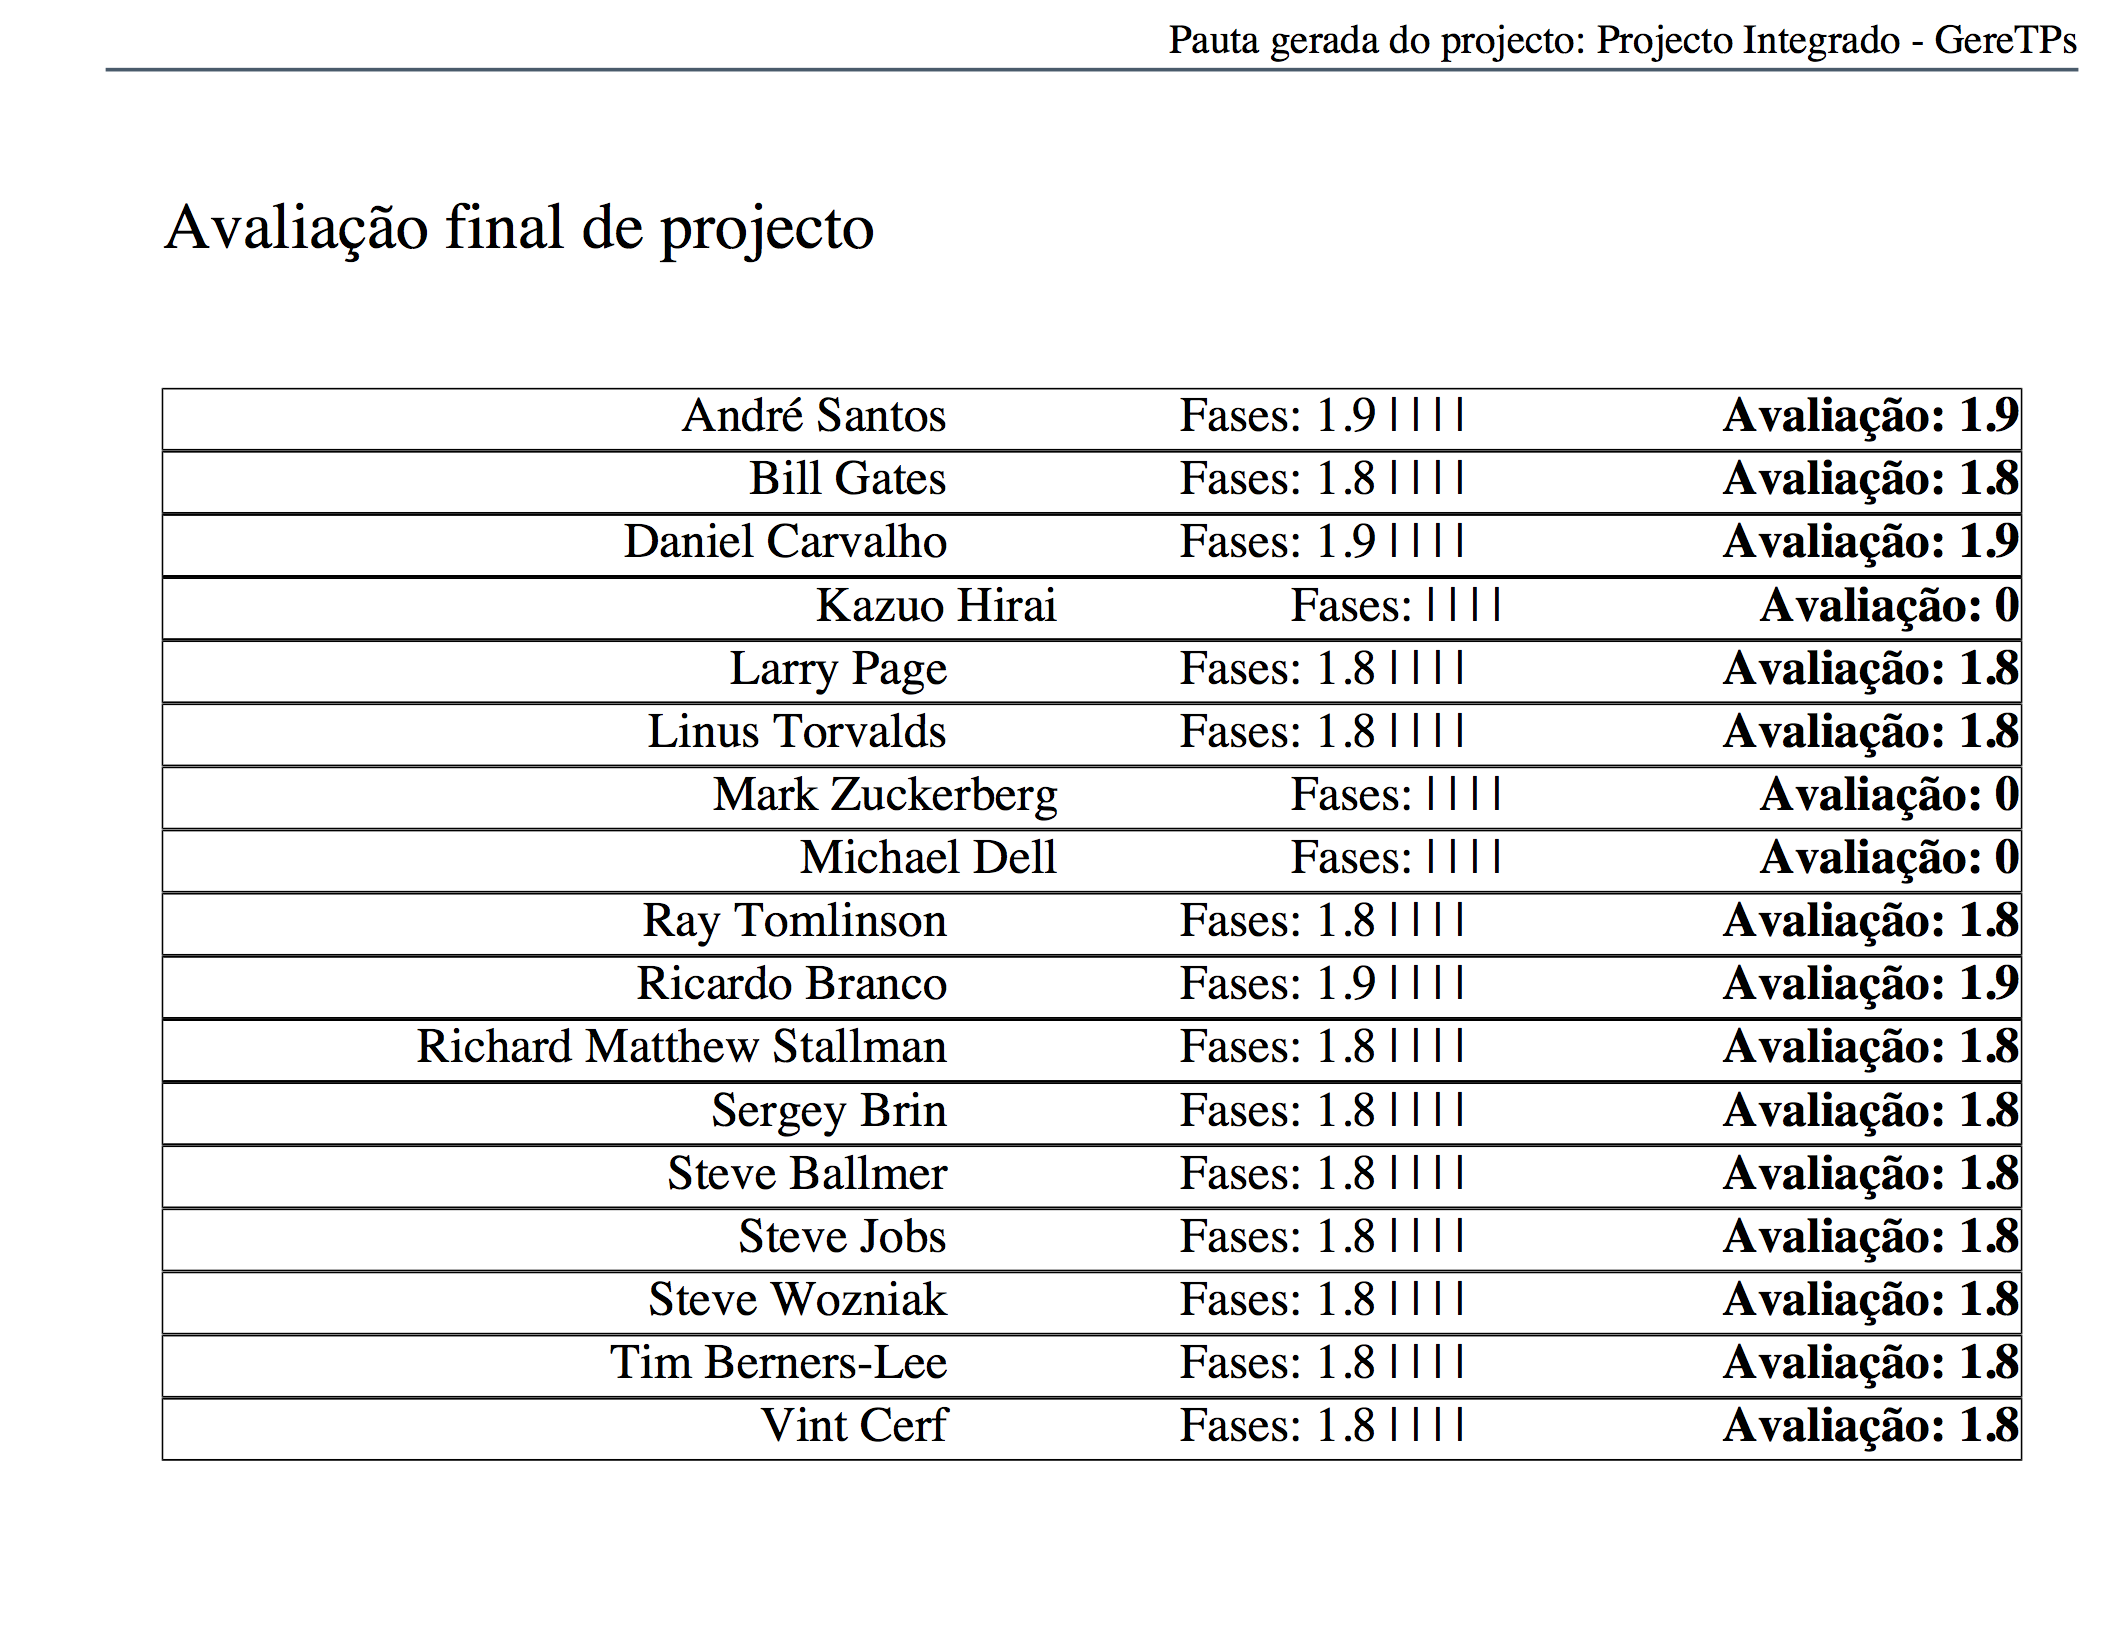
\includegraphics[width=0.7\textwidth,center]{images/implementacao/pauta1}
  \caption{Exportação XSLFO para PDF}
  \label{fig:pauta1}
\end{figure}

\begin{figure}[H]
  \centering
  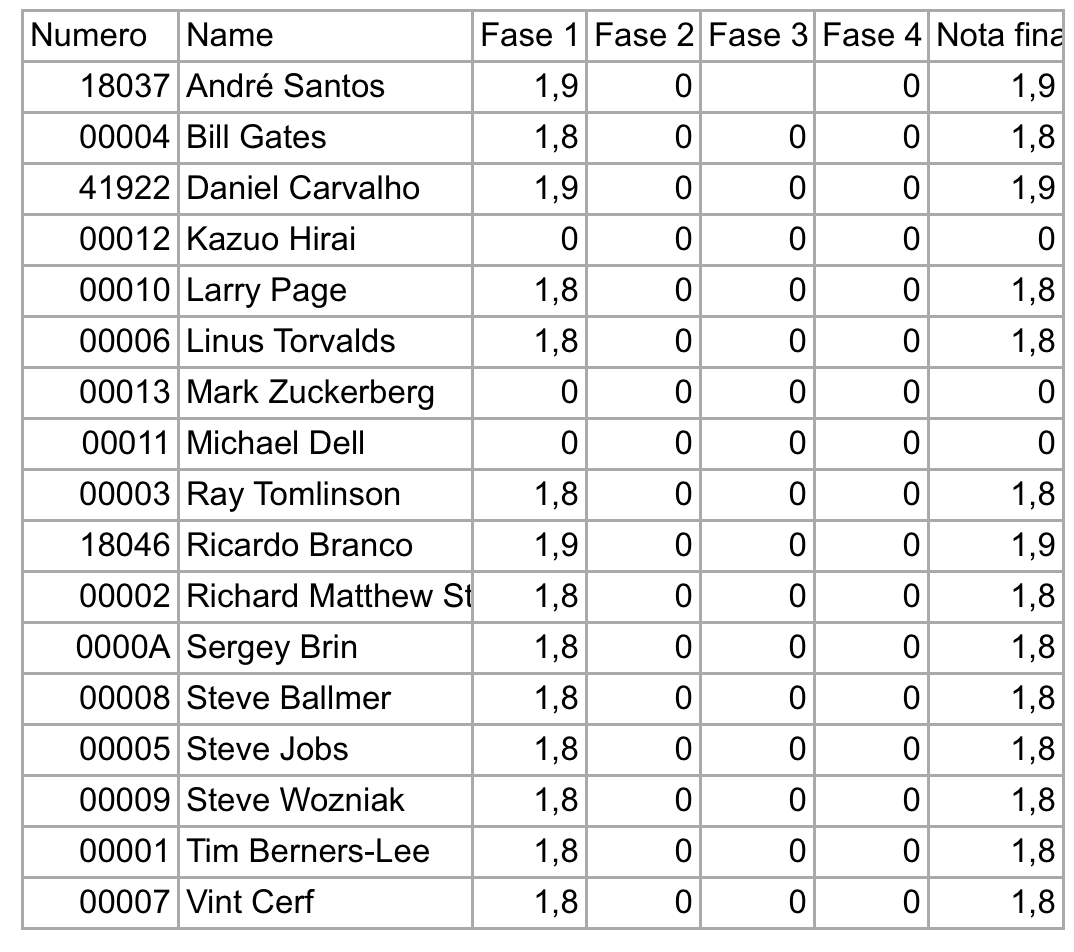
\includegraphics[width=0.7\textwidth,center]{images/implementacao/pauta2}
  \caption{Exportação para XLS}
  \label{fig:pauta2}
\end{figure}